%%*************************************************************************%%
%%  SCALASCA    http://www.scalasca.org/                                   %%
%%*************************************************************************%%
%%  Copyright (c) 1998-2019                                                %%
%%  Forschungszentrum Juelich GmbH, Juelich Supercomputing Centre          %%
%%                                                                         %%
%%  Copyright (c) 2009-2014                                                %%
%%  German Research School for Simulation Sciences GmbH,                   %%
%%  Laboratory for Parallel Programming                                    %%
%%                                                                         %%
%%  This software may be modified and distributed under the terms of       %%
%%  a BSD-style license.  See the COPYING file in the package base         %%
%%  directory for details.                                                 %%
%%*************************************************************************%%



\documentclass[a4paper]{article}


% Include configuration
\include{config}

% Extra packages
\usepackage[USenglish]{babel}
\usepackage{pslatex}
\usepackage{tabularx}
\usepackage{xspace}

% Page & text layout
\usepackage{geometry}
\geometry{twoside=false,a4paper,hmargin={2cm,2cm},vmargin={2cm,2cm}}
\setlength{\parindent}{0cm}
\setlength{\headheight}{34pt}
\setlength{\footskip}{15pt}
\renewcommand{\arraystretch}{1.1}

% Headers & footers
\usepackage{fancyhdr}
\pagestyle{fancy}
\makeatletter
\fancyhf{}
\fancyhead[L]{\bfseries\LARGE\@title}
\fancyhead[R]{
\includegraphics[height=2.0\baselineskip]{scalasca_logo}}%
\fancyfoot[L]{Project URL: \texttt{\PackageUrl}}
\fancyfoot[C]{\thepage}
\fancyfoot[R]{Contact/support: \texttt{\PackageBugreport}}
\makeatother
\renewcommand{\footrulewidth}{\headrulewidth}

% Graphics
\usepackage{graphicx}

% Shortcuts
\newcommand{\Version}{v\PackageMajor.\PackageMinor\xspace}
\newcommand{\Scalasca}{\textsc{Scalasca}\xspace}
\newcommand{\Scorep}{\textsc{Score-P}\xspace}
\newcommand{\Cube}{\textsc{Cube}\xspace}

% Document setup
\title{\Scalasca \Version Quick Reference}


\begin{document}

%--- GENERAL ----------------------------------------------------------------

\subsection*{General}

\begin{itemize}
  \item \Scalasca is an open-source toolset for scalable performance analysis of
        large-scale parallel applications.
  \item \Scalasca uses the community measurement system \Scorep to generate profiles and
        tracing results.
  \item Use the \textbf{\texttt{scorep}}  and \textbf{\texttt{scalasca}} commands with
        appropriate action flags to
        \textit{instrument\/} application object files and executables,
        \textit{analyze\/} execution measurements, and interactively
        \textit{examine\/} measurement/analysis experiment archives.
  \item For short usage explanations, use \Scalasca commands without arguments,
        or add `\textbf{\texttt{-v}}' for verbose commentary.
  \item View possible parameters for the \Scorep instrumenter by calling
        \textbf{\texttt{scorep --help}}
\end{itemize}

%--- INSTRUMENTATION --------------------------------------------------------

\subsection*{\Scorep Instrumentation}
\begin{itemize}
  \item Prepend \textbf{\texttt{scorep}} and any instrumentation flags to your
        compile/link commands.  Alternatively, use the \Scorep compiler wrappers.
  \item Additional options to the instrumenter must be specified
        \textit{before} the compiler/linker command.
  \item By default, MPI and OpenMP operations are automatically instrumented, and
        many compilers are also able to instrument all routines found in source files
        (unless explicitly disabled with \textbf{\texttt{--nocompiler}}).
  \item To enable manual instrumentation (described on page \pageref{sec:manual_inst})
        using the user instrumentation API, add \textbf{\texttt{--user}},
        and/or using \textsc{pomp} directives, add \textbf{\texttt{--pomp}}.
  \item To enable automatic source-to-source function instrumentation with PDToolkit, use \textbf{\texttt{--pdt}}.
  \item To enable CUDA instrumentation use \textbf{\texttt{--cuda}}.
  \item Examples: \\
    \begin{minipage}[t]{0.4\linewidth}
      Original command: \\\ttfamily
      mpicc -c foo.c \\
      mpicxx -o foo foo.cpp \\
      mpif90 -openmp -o bar bar.f90
    \end{minipage}
    \begin{minipage}[t]{0.59\linewidth}
      \Scorep instrumentation command: \\\ttfamily
      \textbf{scorep} mpicc -c foo.c \\
      \textbf{scorep --user} mpicxx -o foo foo.cpp \\
      \textbf{scorep} mpif90 -openmp -o bar bar.f90
    \end{minipage}
  \item Often it is preferable to prefix Makefile compile/link commands
        with \texttt{\$(PREP)} and set \texttt{PREP="scorep"} for
        instrumented builds (leaving \texttt{PREP} unset for uninstrumented builds).
\end{itemize}


%--- MEASUREMENT / ANALYSIS -------------------------------------------------

\subsection*{Measurement \& Analysis}
\begin{itemize}
  \item Prepend \textbf{\texttt{scalasca -analyze}} (or \textbf{\texttt{\em scan}})
        to the usual execution command line to perform a measurement with
        \Scalasca runtime summarization and associated automatic trace analysis
        (if applicable).
  \item \Scorep instrumented applications can be run without prefix, using only
        environment variables for control. In this case the trace analysis won't
        be started automatically.
  \item To reuse an existing measurement for analysis, add the flag \textbf{\texttt{-a}}.
  \item Each measurement is stored in a new experiment archive
        which is not overwritten by a subsequent measurement.
  \item By default, only a runtime summary (profile) is collected
        (equivalent to specifying \textbf{\texttt{-s}}).
  \item To enable trace collection \& analysis, add the flag \textbf{\texttt{-t}}.
  \item An archive directory name can be explicitly specified with
        \textbf{\texttt{scan -e {\em title}}}.
  \item To analyze MPI and hybrid OpenMP+MPI applications,
        use the usual MPI launcher command and arguments.
  \item To analyze serial and (pure) OpenMP applications, omit the MPI launcher
        command.
  \item Examples:\\
    \begin{minipage}[t]{0.255\linewidth}
      Original command: \\\ttfamily
      mpiexec -np 4 foo args \\
      OMP\_NUM\_THREADS=3 bar \\
      mpiexec -np 4 foobar
    \end{minipage}
    \begin{minipage}[t]{0.5\linewidth}
      \Scalasca measurement \& analysis command: \\\ttfamily
      \textbf{scalasca -analyze} mpiexec -np 4 foo args \\
      OMP\_NUM\_THREADS=3 \textbf{scan -t} bar \\
      \textbf{scan -s} mpiexec -np 4 foobar
    \end{minipage}
    \begin{minipage}[t]{0.325\linewidth}
      Experiment archive: \\\ttfamily
      \# scorep\_foo\_4\_sum \\
      \# scorep\_bar\_Ox3\_trace \\
      \# scorep\_foobar\_4x3\_sum \\
      \# (w/ 3 OpenMP threads)
    \end{minipage}
\end{itemize}


\subsubsection*{Measurement configuration}

Measurement is controlled by a number of variables which can be set through
corresponding environment variables: the configuration is stored in the
experiment archive as \texttt{scorep.cfg}. The most important variables are:
\\[1ex]
\begin{tabularx}{\linewidth}{lX@{\hspace*{10mm}}l}
  \textbf{Variable} & \textbf{Purpose} & \textbf{\Scorep default} \\

  \texttt{SCOREP\_EXPERIMENT\_DIRECTORY} &
    Experiment archive title, explicitly specified by \texttt{-e} or
    automatically given a reasonable name if not specified.
    &
    \texttt{scorep-}\textit{timestamp} \\

   \texttt{SCOREP\_ENABLE\_PROFILING} &
    Enabling or disabling profile generation.
    &
    true \\

   \texttt{SCOREP\_ENABLE\_TRACING} &
    Enabling or disabling trace generation.
    &
    false \\

 \texttt{SCOREP\_FILTERING\_FILE} &
    Name of file containing a specification of functions which should be
    ignored during measurement.
    &
    --- \\

   \texttt{SCOREP\_VERBOSE} &
    Controls generation of additional (debugging) output by measurement
    system. &
    false \\

  \texttt{SCOREP\_TOTAL\_MEMORY} &
    Size of per-process memory reserved for \Scorep in bytes. &
    16\,384\,000 \\
\end{tabularx}
\\[1ex]
The full list of supported configuration variables and their values can be retrieved using
\texttt{scorep-info config-vars --full}.

%--- Score-P ----------------------------------------------------------

\subsection*{\Scorep experiment archives -- typical directory content}

    \begin{tabularx}{\linewidth}{lX}
      \textbf{File} & \textbf{Description} \\
        \texttt{profile.cubex} &
                Analysis report of runtime summarization. \\
        \texttt{scorep.cfg} &
                Measurement configuration when the experiment was collected.\\
        \texttt{scorep.log} &
                Output of the instrumented program and measurement system.\\
        \texttt{scout.cubex} &
                Intermediate analysis report of the parallel trace analyzer.\\
        \texttt{scout.log} &
                 Output of the parallel trace analyzer.\\
       \texttt{summary.cubex} &
                Post-processed analysis report of runtime summarization.
                (May include HWC metrics.)\\
        \texttt{trace.cubex} &
                Post-processed analysis report of the trace analyzer.
                (Does not include HWC metrics.)\\
        \texttt{trace.stat} &
                Most-severe pattern instances and pattern statistics.\\
        \texttt{traces/} &
                Sub-directory containing event traces for each process/thread.\\
        \texttt{traces.def/.otf2} &
                Definitions and anchor files for the event traces.\\
    \end{tabularx}

\subsubsection*{Determining trace buffer capacity requirements}
Based on an analysis report, the required trace buffer capacity can be
estimated using
\begin{flushright}
  \fbox{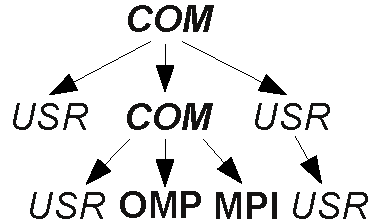
\includegraphics[width=28mm]{score_tree}}\\
  \vspace*{-22mm}
\end{flushright}
\begin{center}
  \ttfamily
  scorep-score [-r] [-f \textit{\rmfamily filter\_file}]
               \textit{\rmfamily experiment\_archive}/profile.cubex
\end{center}
\begin{itemize}
  \item To get detailed information per region (i.e., function or subroutine), use
        \texttt{-r}
  \item To take a proposed filter file into account, use
        \texttt{-f \textit{\rmfamily filter\_file}}
  \item The report specifies the maximum estimated
        required memory per process, which can be used to set\\
        \texttt{SCOREP\_TOTAL\_MEMORY} appropriately to avoid intermediate flushes
        in subsequent tracing experiments.
\end{itemize}

% first column
\begin{minipage}[t]{0.5\textwidth}
The \Scorep filter format allows to include and exclude functions from measurement
using their names with possible use of wildcards.
The respective commands are processed in sequence, allowing for hierarchical inclusion-exclusion schemes.
To the right is an example for a standard filter file.
\end{minipage}
\begin{minipage}[t]{0.49\textwidth}
\ttfamily
 \hspace*{2ex} SCOREP\_REGION\_NAMES\_BEGIN \\
 \hspace*{5ex}   EXCLUDE \\
 \hspace*{9ex}     binvcrhs*  \\
 \hspace*{9ex}     matmul\_sub*  \\
 \hspace*{2ex} SCOREP\_REGION\_NAMES\_END
\end{minipage}

\subsection*{\Cube{4} algebra and utilities}

Uniform behavioural encoding, processing and interactive examination of
parallel application execution analysis reports.

\begin{itemize}
  \item \Cube{4} provides a variety of utilities
  for differencing, combining and other operations on analysis reports, e.g.,
  \texttt{cube\_diff}, \texttt{cube\_mean}, \texttt{cube\_merge}.
  \item \texttt{cube\_cut} can be used to prune uninteresting
call-trees and/or re-root with a specified call-tree node.
  \item \texttt{cube\_stat} can be used to produce custom statistical reports in CSV or plain text format.
  \item \texttt{cube\_topoassist} can be used to add or modify topology specifications.
\end{itemize}

\clearpage

%--- ANALYSIS REPORT EXAMINATION (Qt version) -------------------------------

\subsection*{Analysis Report Examination}
\begin{itemize}
  \item To interactively examine the contents of a \Scalasca experiment,
        after final processing of runtime summary and trace analysis,
        use \textbf{\texttt{scalasca -examine}} (or \textbf{\texttt{\em square}}) with the
        experiment archive directory name as argument.
  \item To skip the graphical user interface and get a textual score output (using the
        \texttt{scorep-score} utility), add the \textbf{\texttt{-s}} flag.
  \item If multiple analysis reports are available,
        a trace analysis report is shown in preference to a runtime
        summary report: other reports can be specified directly or selected
        from the File/Open menu.
  \item Results are displayed using three coupled tree browsers showing
    \begin{itemize}
      \setlength{\itemsep}{0cm}
      \item Metrics (i.e., performance properties/problems)
      \item Call-tree or flat region profile
      \item System location (alternative: graphical displays, such as
            box/violin plot, Sunburst view, or physical/virtual Cartesian
            topologies. Topologies with more than 3 dimensions will be folded).
    \end{itemize}
\end{itemize}

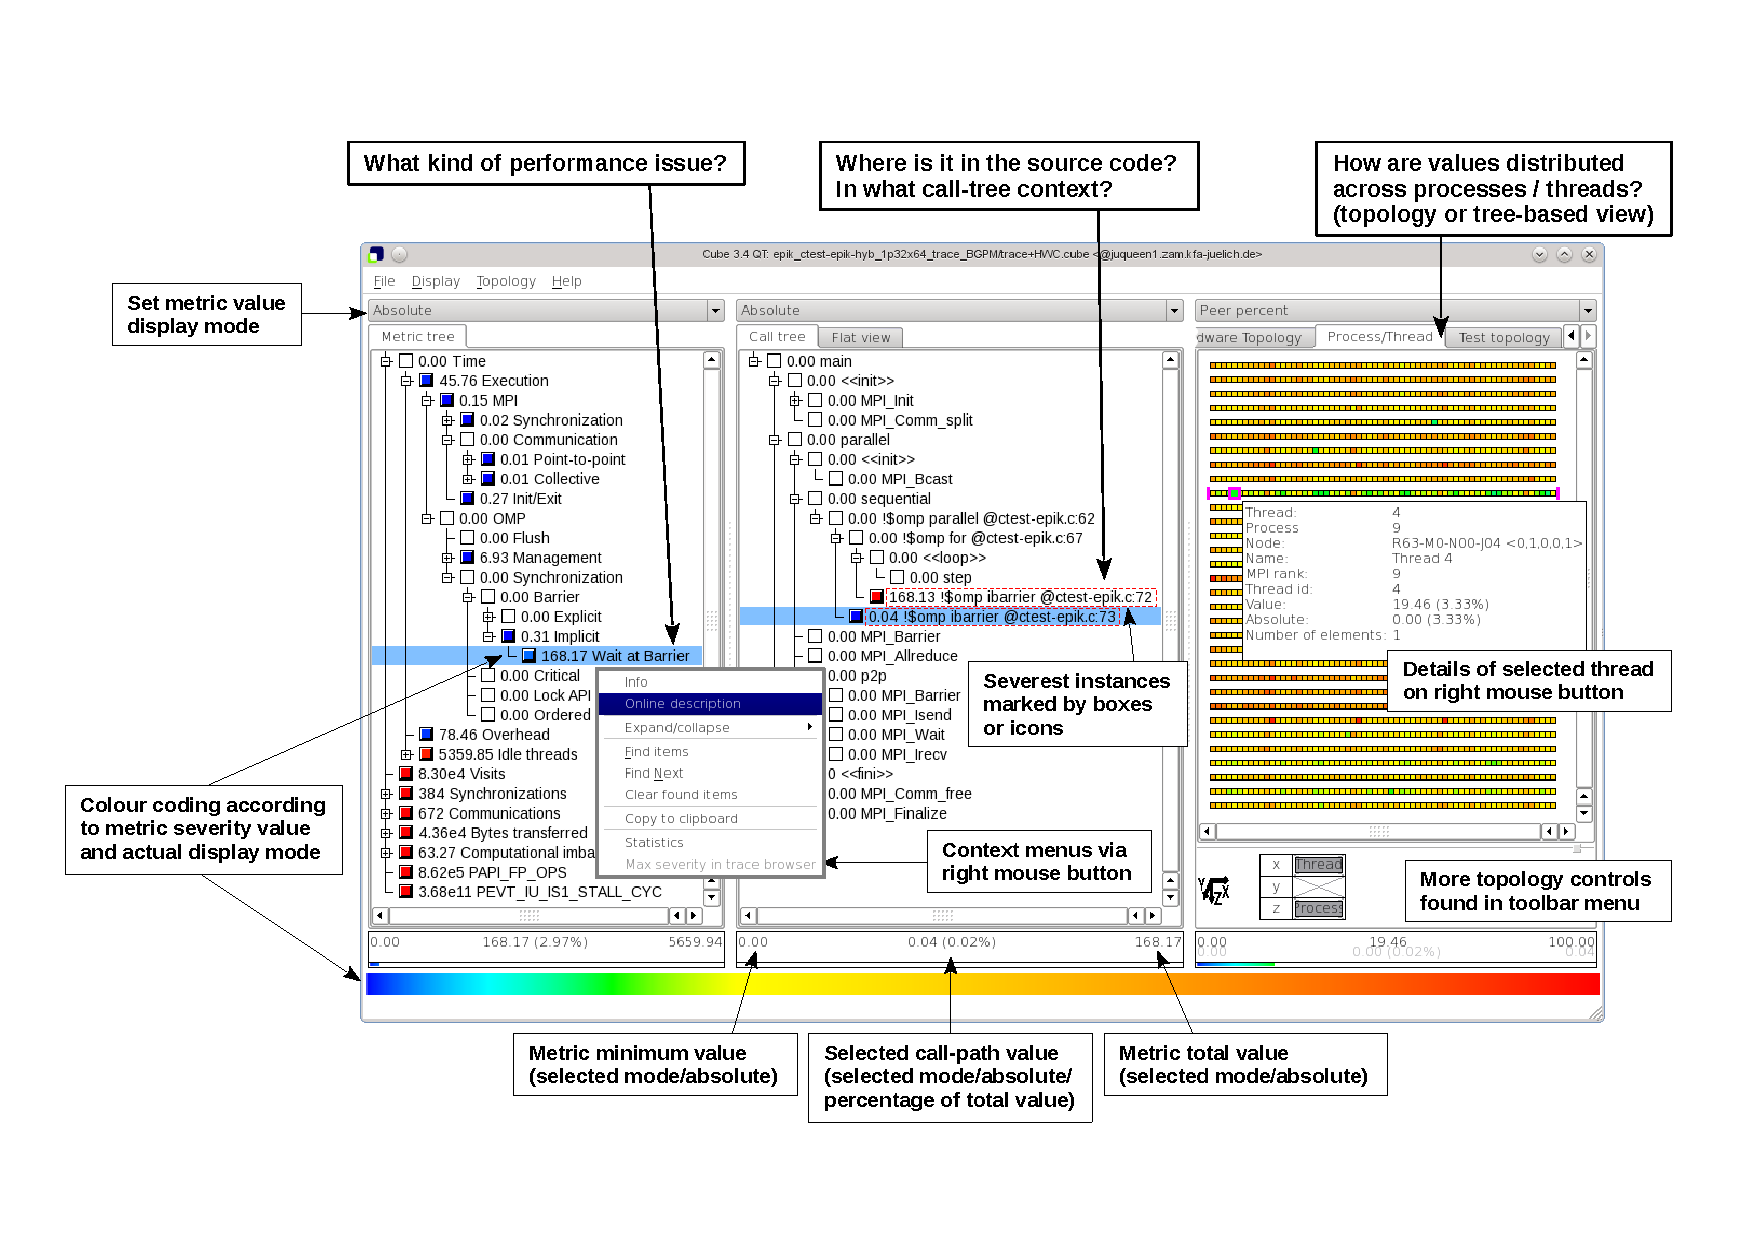
\includegraphics[viewport=31 56 803 528,clip,width=\linewidth]{ctest-epik-hyb}

\vspace*{-2mm}
\begin{itemize}
  \item Analyses are presented in trees, where collapsed nodes represent
{\em inclusive\/} values (consisting of the value of the node itself and all of
its child nodes), which can be selectively expanded to reveal {\em exclusive\/}
values (i.e., the node `self' value) and child nodes.
  \item When a node is selected from any tree,
        its {\em severity\/} value (and percentage) are shown in the panel below it,
        and that value distributed across the tree(s) to the right of it.

  \item Selective expansion of critical nodes, guided by the
color scale, can be used to hone in on performance problems.

  \item Each tree browser provides additional information via a context menu
        (on the right mouse button), such as the description of the selected metric
        or source code for the selected region (where available).
  \item Metric severity values can be displayed in various modes: \\[1ex]
    \begin{tabularx}{\linewidth}{lX}
      \textbf{Mode} & \textbf{Description} \\

      Absolute &
        Absolute value in the corresponding unit of measurement. \\

      Root percent &
        Percentage relative to the inclusive value of the root node of the
        corresponding hierarchy. \\

      Selection percent &
        Percentage relative to the value of selected node in corresponding
        tree browser to the left. \\

      Peer percent &
        Percentage relative to the maximum of all peer values (all values of
        the current leaf level). \\

      Peer distribution &
        Percentage relative to the maximum and non-zero minimum of all peer
        values. \\

      External percent &
        Similar to ``Root percent,'' but reference values are taken from
        another experiment.
    \end{tabularx}
\end{itemize}

\clearpage


%--- MANUAL INSTRUMENTATION --------------------------------------------

\subsection*{Manual source-code instrumentation}
\label{sec:manual_inst}

\begin{itemize}
  \item Region or phase annotations manually inserted in source files can augment or
substitute automatic instrumentation, and can improve the structure of analysis reports
to make them more readily comprehensible.
  \item These annotations can be used to mark any sequence
or block of statements, such as functions, phases, loop nests, etc., and can be
nested, provided that \emph{every enter has a matching exit}.
  \item If automatic compiler instrumentation is not used (or not
available), it is typically desirable to manually instrument at least
the \texttt{main} function/program and perhaps its major phases (e.g.,
initialization, core/body, finalization).
\end{itemize}

\subsection*{{\sc Score-P} user instrumentation API}
\label{sec:Scorep_inst}
    \begin{minipage}[t]{0.49\linewidth}
      C/C++: \\\ttfamily
      \#include <scorep/SCOREP\_User.h> \\
      ... \\
      void foo() \{ \\
      \hspace*{1ex} ... // local declarations \\
      \hspace*{1ex} SCOREP\_USER\_FUNC\_BEGIN(); \\
      \hspace*{1ex} ... // executable statements \\
      \hspace*{1ex} if (...) \{ \\
      \hspace*{2ex} SCOREP\_USER\_FUNC\_END(); \\
      \hspace*{2ex} return; \\
      \hspace*{1ex} \} else \{ \\
      \hspace*{2ex} SCOREP\_USER\_REGION\_DEFINE(r\_name); \\
      \hspace*{2ex} SCOREP\_USER\_REGION\_BEGIN(r\_name, "bar", \\
      \hspace*{10ex} SCOREP\_USER\_REGION\_TYPE\_COMMON); \\
      \hspace*{2ex} ... \\
      \hspace*{2ex} SCOREP\_USER\_REGION\_END(r\_name); \\
      \hspace*{1ex} \} \\
      \hspace*{1ex} ... // executable statements \\
      \hspace*{1ex} SCOREP\_USER\_FUNC\_END(); \\
      \}
    \end{minipage}
    \begin{minipage}[t]{0.49\linewidth}
      Fortran: \\\ttfamily
      \#include <scorep/SCOREP\_User.inc> \\
      ... \\
      subroutine foo \\
      \hspace*{1ex} ... ! local declarations \\
      \hspace*{1ex} SCOREP\_USER\_FUNC\_DEFINE() \\
      \hspace*{1ex} SCOREP\_USER\_REGION\_DEFINE(r\_name) \\
      \hspace*{1ex} SCOREP\_USER\_FUNC\_BEGIN("foo") \\
      \hspace*{1ex} ... ! executable statements \\
      \hspace*{1ex} if (...) then \\
      \hspace*{2ex} SCOREP\_USER\_FUNC\_END() \\
      \hspace*{2ex} return \\
      \hspace*{1ex} else \\
      \hspace*{1ex} SCOREP\_USER\_REGION\_BEGIN(r\_name, "bar", \\
      \hspace*{9ex} SCOREP\_USER\_REGION\_TYPE\_COMMON) \\
      \hspace*{1ex} ... \\
      \hspace*{2ex} SCOREP\_USER\_REGION\_END(r\_name) \\
      \hspace*{1ex} end if \\
      \hspace*{1ex} SCOREP\_USER\_FUNC\_END() \\
      end subroutine foo
    \end{minipage}

\begin{itemize}
  \item \texttt{SCOREP\_USER\_FUNC\_BEGIN} and \texttt{SCOREP\_USER\_FUNC\_END} are
provided explicitly to mark the entry and exit(s) of functions/subroutines.
  \item Function names are automatically provided by C/C++, however, in
annotated Fortran functions/subroutines an appropriate name should be
registered with \texttt{SCOREP\_USER\_FUNC\_BEGIN("func\_name")}.
  \item Region identifiers (e.g., \texttt{r\_name}) should be registered
with \texttt{SCOREP\_USER\_REGION\_DEFINE} in each annotated prologue before use with
\texttt{SCOREP\_USER\_REGION\_BEGIN} and \texttt{SCOREP\_USER\_REGION\_END} in the associated body.
  \item Every exit/break/continue/return/etc.{} out of each annotated region
must have corresponding \texttt{\_END()} annotation(s).
  \item Source files annotated in this way need to be compiled with the
\texttt{--user} flag given to the \Scorep instrumenter, otherwise the
annotations are ignored. Fortran source files need to be preprocessed
(e.g., by FPP or CPP).
\end{itemize}

\subsubsection*{{\sc pomp} user instrumentation API}
\label{sec:pomp_inst}

{\sc pomp} annotations provide a mechanism for preprocessors (such as
{\sc opari2}) to conditionally insert user instrumentation.

    \begin{minipage}[t]{0.5\linewidth}
      C/C++: \\\ttfamily
      \#pragma pomp inst init // once only, in main \\
      ... \\
      \#pragma pomp inst begin(name) \\
      \hspace*{2ex} ... \\
      \hspace*{2ex} [ \#pragma pomp inst altend(name) ] \\
      \hspace*{2ex} ... \\
      \#pragma pomp inst end(name)
    \end{minipage}
    \begin{minipage}[t]{0.5\linewidth}
      Fortran: \\\ttfamily
      !POMP\$ INST INIT !~once only, in main program \\
      ... \\
      !POMP\$ INST BEGIN(name) \\
      \hspace*{2ex} ... \\
      \hspace*{2ex} [ !POMP\$ INST ALTEND(name) ] \\
      \hspace*{2ex} ... \\
      !POMP\$ INST END(name)
    \end{minipage}

\begin{itemize}
  \item Every intermediate exit/break/return/etc.{} from each annotated region
must have an \texttt{altend} or \texttt{ALTEND} annotation.
  \item Source files annotated in this way need to be processed with the
\texttt{--pomp} flag given to the \Scorep instrumenter, otherwise the
annotations are ignored.
\end{itemize}


\clearpage



%--- Tips ---------------------------------------------------------

\subsection*{Tips for effective use of the \Scalasca toolset}

\begin{enumerate}

\item Determine one or more repeatable execution configurations (input
data, number of processes/threads) and time their overall execution to
have a baseline for reference.  (If possible, also identify maximum
memory requirements.)
\begin{itemize}
\item Ensure that the execution terminates cleanly, e.g., with
    \verb+MPI_Finalize+ and not calling \texttt{STOP} or
    \texttt{exit(\mbox{\rmfamily\itshape val})}.
\item Excessively long execution durations can make
measurement and analysis inconvenient, therefore the test configuration
shouldn't be longer than sufficient to be representative.
\end{itemize}

\item Modify the application build procedure (e.g., Makefile) to prepend the
\Scorep instrumenter to compile and link commands, and produce an
instrumented executable.

\begin{itemize}
\item MPI library calls and OpenMP parallel regions will be instrumented by
default, along with user functions if supported by the compiler.
\item Serial libraries and source modules using neither MPI nor OpenMP
are generally not worth instrumenting with \Scorep, and indeed may result in
undesirable measurement overheads.
\end{itemize}

\item Prefix the usual launch/run command with the \Scalasca analyzer to
run the instrumented executable under control of the \Scalasca
measurement collection and analysis nexus to produce an experiment
archive directory.

\begin{itemize}
\item By default the experiment archive is produced in the current
working directory, and its name will start with `\verb+scorep_+' followed
by some configuration descriptors if created automatically.
The \Scalasca measurement \& analysis nexus automatically
generates a default experiment title from the target executable, compute node
mode (if appropriate), number of MPI processes (or \texttt{O} if
omitted), number of OpenMP threads (if \texttt{OMP\_NUM\_THREADS} is set),
summarization or tracing mode, and optional metric specification.
\item If a similarly configured experiment has already been run and its
archive directory blocks new measurement experiments.
\item If no path is given, e.g., in a run without \Scalasca, the name will
start with `\verb+scorep-+' followed by an unique identifier (timestamp).
In this mode an existing archive is renamed with an unique
suffix unless specified otherwise.
\item A call-path profile summary report containing Time and Visits metrics
(and when appropriate also MPI file I/O and message statistics and
hardware counters) for each process/thread is produced by default.
\item If the (default) measurement configuration is inadequate for a
complete measurement to be collected, warnings will indicate that
one or more configuration variables should be adjusted (e.g.,
\verb+SCOREP_TOTAL_MEMORY+).
\item Compare the runtime to the (uninstrumented) reference to
estimate implicit instrumentation dilation overhead.
\end{itemize}

\item Use the \Scalasca examiner to explore the analysis report in the
experiment archive.

\begin{itemize}
\item Uninstrumented or filtered routines will not appear in the
analysis report, and their associated metric severities will be attributed to
the last measured routine from which they are called (as if they were `inlined').
\item Additional structure can be included in the analysis report by
using the Score-P user instrumentation API to specify (nested) regions or phases
as annotations in the source code.
\end{itemize}

\item Score the quality of the summary analysis report (particularly if
dilation is significant),  adjust measurement configuration using a
filter file, adjust OpenMP instrumentation, or selectively instrument
source modules (or routines).

\begin{itemize}
\item Investigate use of a filter file specifying instrumented routines
to be ignored during measurement collection.
\item Routines with very high visit counts and relatively low total
times (which are not MPI functions and OpenMP parallel regions)
are appropriate candidates for filtering, and can be identified from the
flat profile view in the GUI, or score reports generated with
`\verb+scalasca -examine -s+' or using `\verb+scorep_score -r+'.
\item Highly-recursive functions are typically also worth removing:
recursion is often indicated by a large maximum call path depth.
\item A prospective filter file can be specified to scoring with '\verb+-f+'
for evaluation prior to being used to re-do measurement and re-check dilation.
\item Some routines might still present excessive overhead even when
filtered, and these should not be instrumented.  The build
procedure may need to be adjusted not to prefix the \Scorep
instrumenter when compiling the associated source modules.
When \Scorep is configured with PDToolkit, it can be used to selectively instrument
entire source modules or individual routines (see PDToolkit documentation for details).
\end{itemize}

\item Use scoring on the (revised/filtered) summary analysis report
to determine an appropriate size for the \Scorep memory settings.

\begin{itemize}
\item For the estimated memory requirements per process, the \verb+SCOREP_TOTAL_MEMORY+
environment variable can be adjusted to avoid intermediate buffer flushes.
\item \verb+SCOREP_TOTAL_MEMORY+ should be set after consideration of the
memory available when measuring the instrumented application execution
and the system's I/O and filesystem performance and capacity.  (These
vary enormously from system to system and can quickly be overwhelmed by
large traces!)
\item Additional user routines can be included in a filter file to
reduce trace buffer requirements.
\end{itemize}

\item Repeat measurement specifying the `\verb+-t+' flag to the
\Scalasca analyzer (along with other configuration settings if
necessary) to collect and automatically analyze execution traces.

\begin{itemize}
\item Traces are generally written directly into the experiment archive to
avoid copying at completion.
\item A filesystem capabable of efficient parallel file I/O should be used when available.
\item If there are \Scorep messages reporting trace flushing to disk prior to
closing the experiment, these intermediate flushes are often highly
disruptive.
Enlarging trace buffer sizes and/or adjusting
instrumentation or the measurement filter and/or configuring a shorter
execution (perhaps with fewer iterations or timesteps) may be appropriate.
\item Parallel trace analysis requires several times as much memory as the
size of the respective (uncompressed process) traces, and it is currently not
possible to analyze incomplete traces.  When memory is restricted,
trace sizes should be reduced accordingly.
\item If clock condition violations are reported during trace
analysis, set the \verb+SCAN_ANALYZE_OPTS+ environment variable to
\verb+--time-correct+ to incorporate a logical clock correction step during
analysis.
\item Traces from hybrid OpenMP/MPI application executions are analyzed
in parallel by default.  If an OpenMP-aware trace analyzer is not available,
metrics are only calculated for the master thread of OpenMP teams.
\item After the analysis report has been examined and verified to be
complete, it is generally unnecessary to keep the often extremely large
trace files used to generate it (unless further analysis or conversion
is planned): these are in the \verb+traces+
subdirectory of a trace experiment archive, which can be deleted.
\end{itemize}

\item In addition to interactive exploration of analysis reports with
the \Scalasca examiner, they can be processed with a variety of
\Cube algebra tools and utilities.

\item If you encounter difficulties using \Scorep or \Scalasca to instrument applications,
configuring measurement collection and analysis, or interpreting
analysis reports, contact \texttt{\PackageBugreport} for assistance.

\end{enumerate}

\end{document}
